\documentclass[slidestop,compress]{beamer}
\usepackage[orientation=portrait,size=custom, width=55, height=25, debug]{beamerposter}
\usetheme{simple}

\usepackage{lmodern}
\usepackage[scale=2]{ccicons}

% TODO: 
%   position adjustement
%   change colours
%       

% Watermark background (simple theme)

\begin{document}

\begin{frame}[plain]
\begin{block}{\hspace{90 mm} Rapid Prototyping \hspace{170 mm} Control Development}
\begin{columns}
    \column{.35\textwidth}{
\begin{itemize}
\item Designed for rapid iteration
\item FDM 3D printed main structure
\item Inexpensive COTS components: DC Brushless hobby motors, Intel Edison microcontroller, and Sparkfun ``blocks"
\item Controller code written in \emph{Python}
\end{itemize}
\begin{figure}[!ht]
\centering
{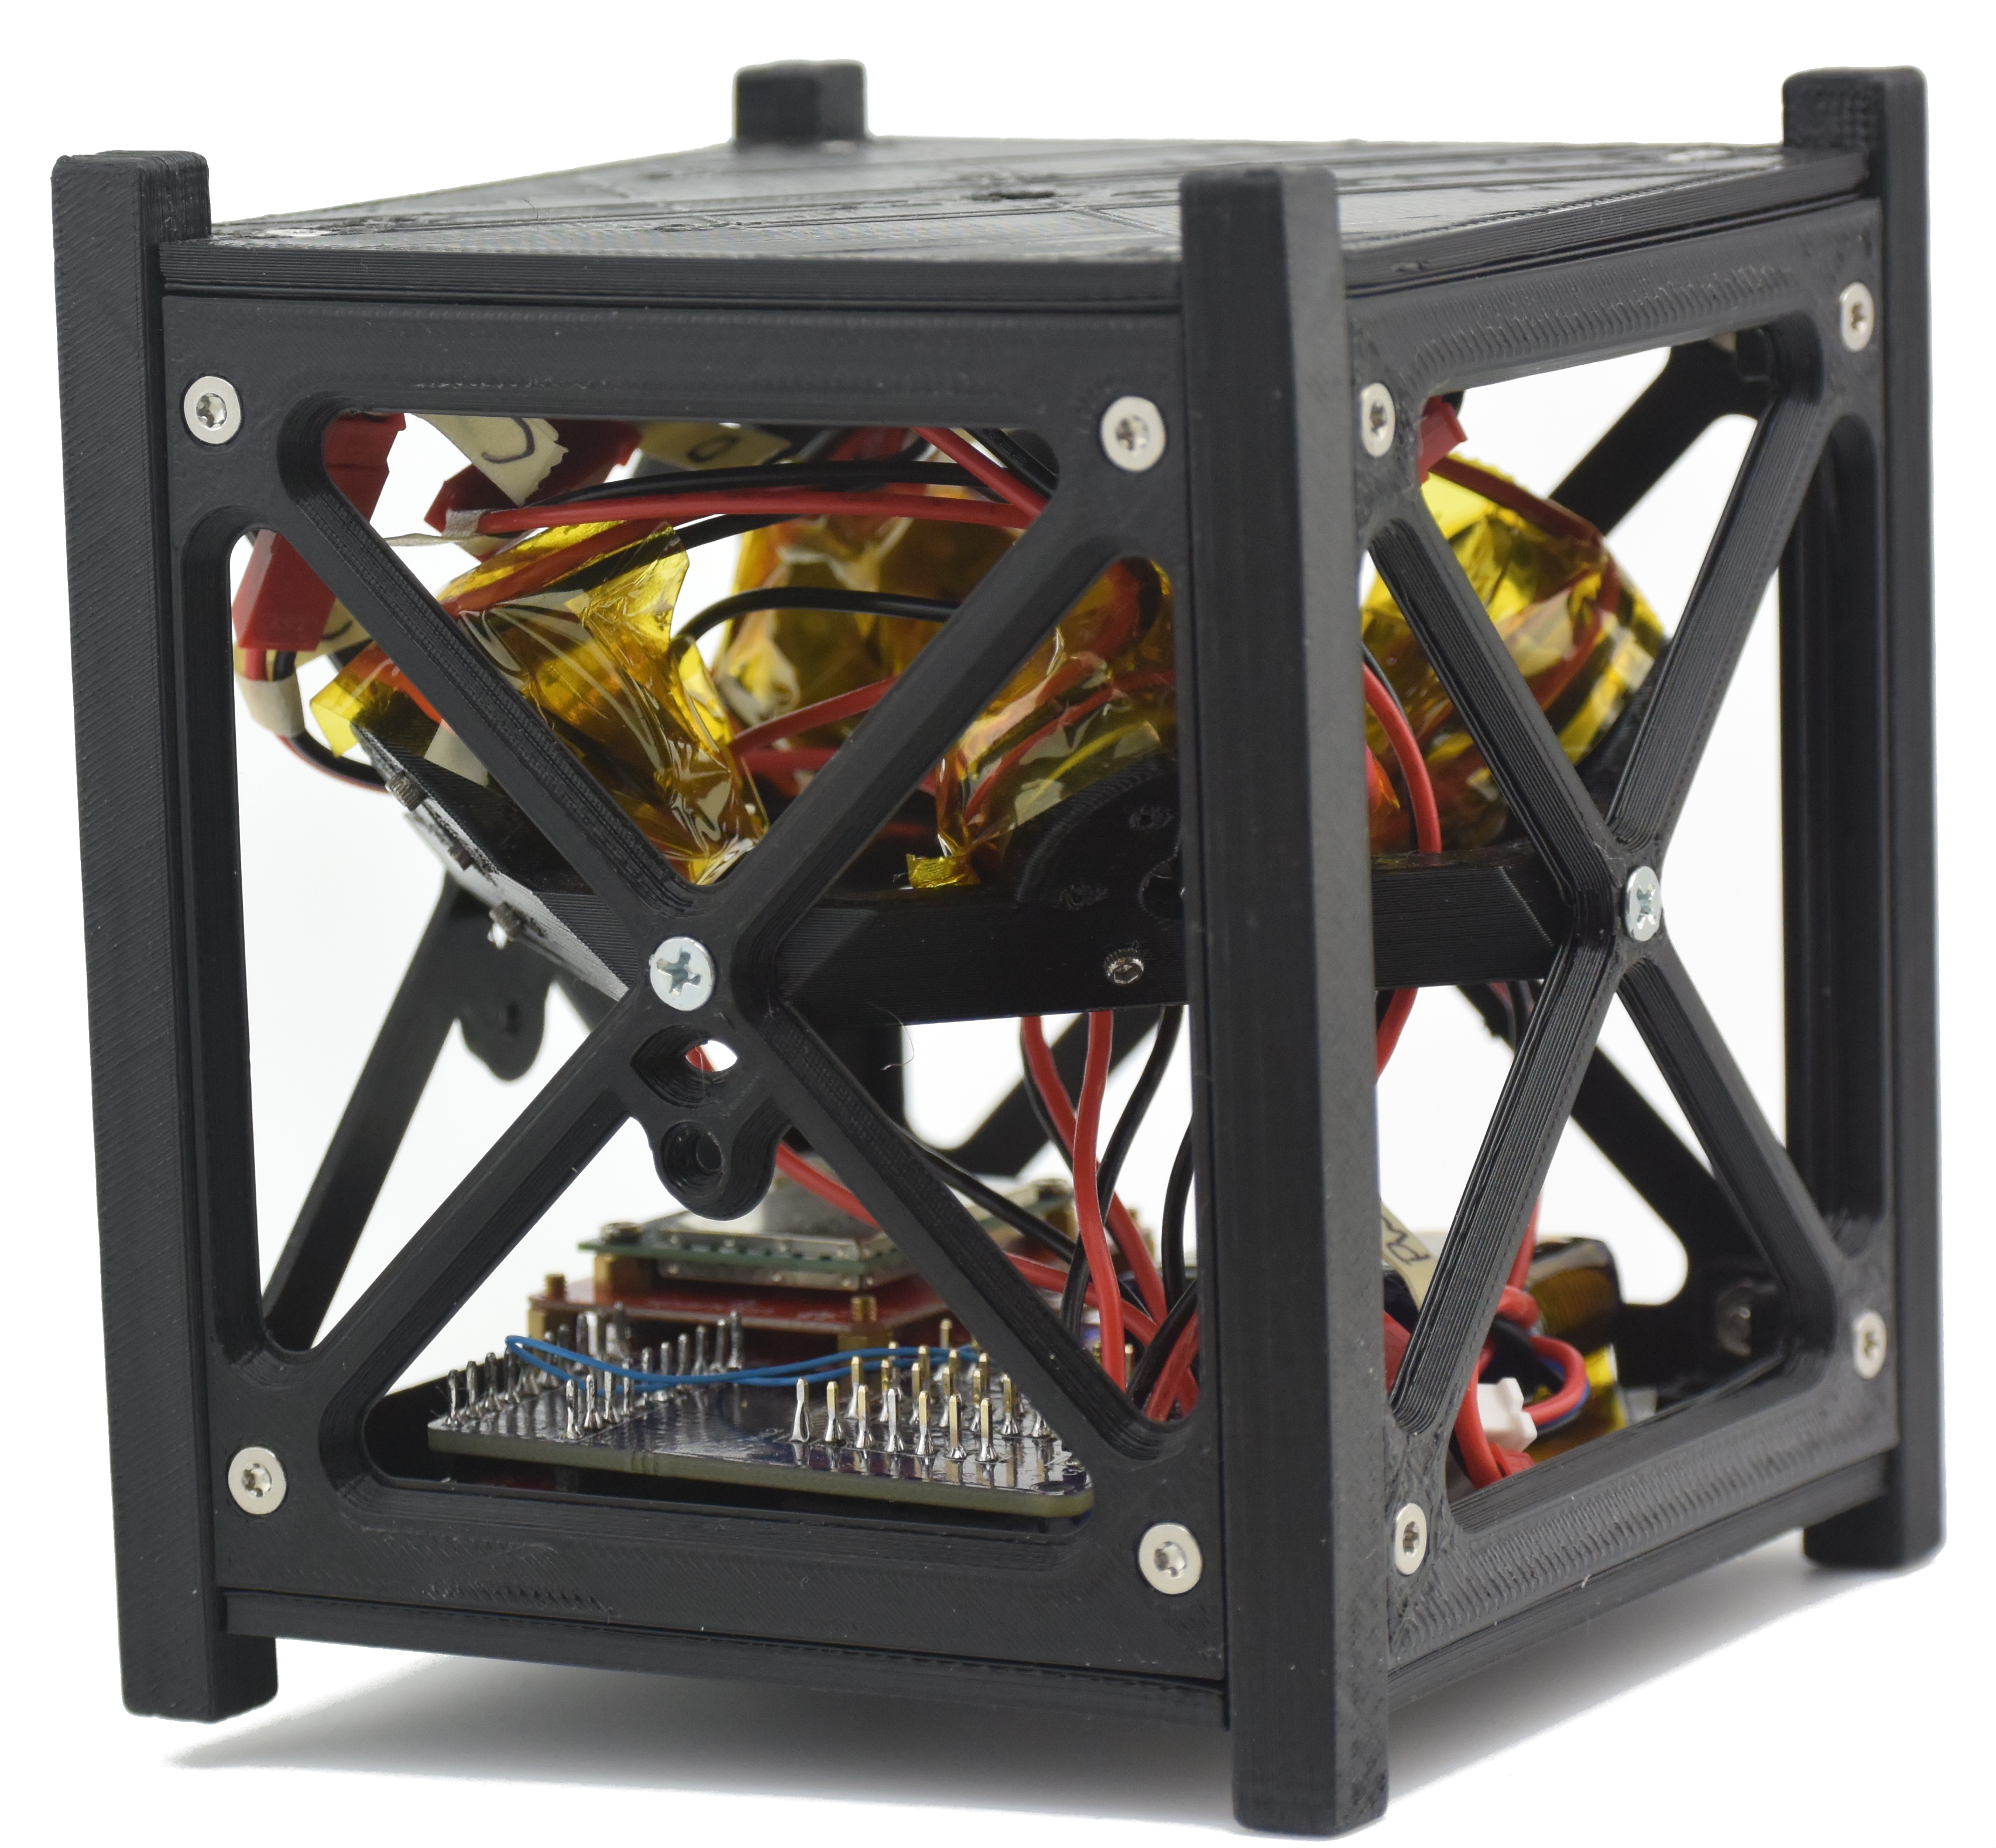
\includegraphics[width=0.7\columnwidth]{DSC_1415.JPG}
\caption{The reaction wheel subsystem test cube.}
} 
\end{figure}}
\hspace{-50 mm} \column{.5\textwidth}
\begin{itemize}
\item The controller for the reaction wheel system is a simple PID loop 
\item The top-level controller design procedure was as follows:
\begin{enumerate}
\item Determine the transfer functions from dynamics analysis of free body diagrams of the system
\item Create simulation in GNU Octave
\item Design the controller using iterative testing (with comparisons to the model) and classical Bode techniques
\end{enumerate}
\item The forces acting on the cube are the torques created by the motors $T_i^0$, damping effects $b_1 \dot{\theta}_{cube}$, and spring effects $G_1 \theta_{cube}$. Summing the moments around the center of gravity gives the following equation (for the x-axis):

\[
\sum M_0^{+ \circlearrowleft} = I_{x,cube} \ddot{\theta}_{x,cube} = T^0_{Ax} + T^0_{Bx} - T^0_{Cx} - T^0_{Dx} + T^0_x - \dot{\theta}_{x,cube} - G_x \theta_{x,cube}.
\] 

\item By setting the system to Standard Equilibrium Position (at SEP the input perturbations are set to zero), considering only a single input, substituting the torque-inertia relation,  and taking the Laplace transform we arrive at the ({\emph{incredibly simple}}) transfer function of the cube:
\[G_A(s)=\frac{\theta_{x,cube}(s)}{\theta_A(s)}=\frac{s^2}{\cfrac{I_{x,cube}}{\sin(45^{\circ}) I_{rw}}s^2 + \cfrac{b_x}{\sin(45^{\circ}) I_{rw}}s + \cfrac{G_x}{\sin(45^{\circ}) I_{rw}}}.
\]
\end{itemize}
\end{columns}
\end{block}    
\end{frame}

\end{document}

